\begin{figure}[H]
  \centering
  \hspace*{-1cm}
  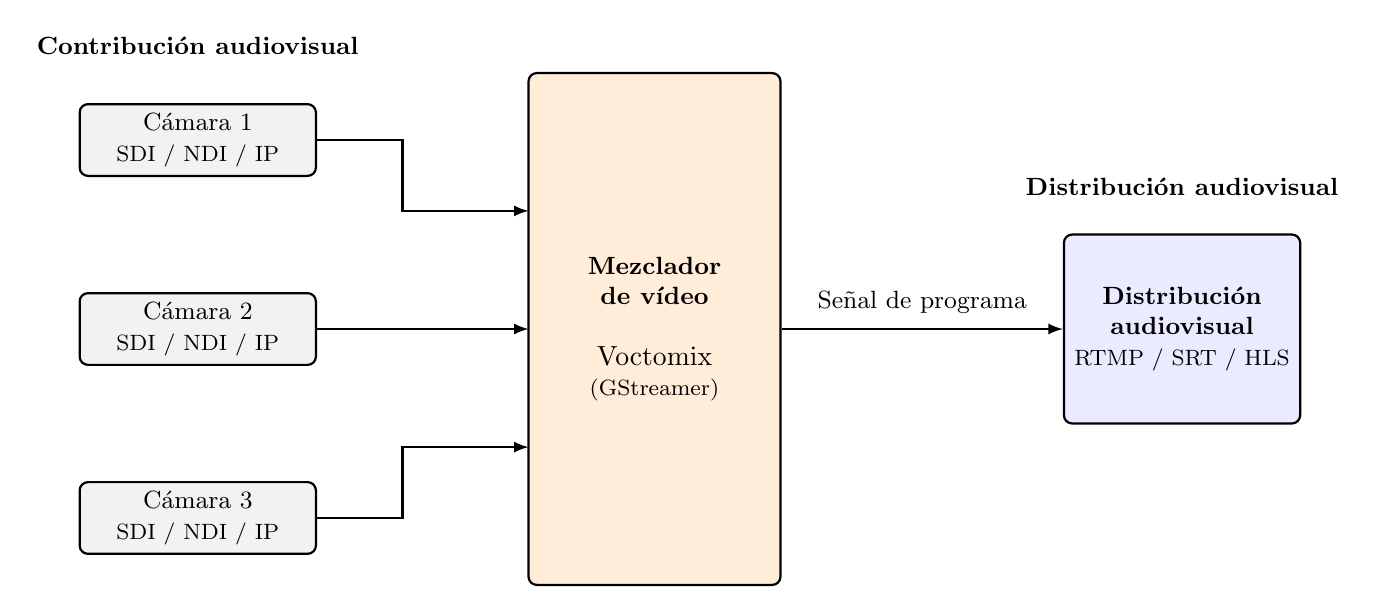
\begin{tikzpicture}[>=latex, thick, font=\small]
    \node[draw, rounded corners=3pt, minimum width=3cm, minimum height=0.9cm,
          align=center, fill=gray!10] (c1) at (0, 2.4) {Cámara 1 \\ {\footnotesize SDI / NDI / IP}};
    \node[draw, rounded corners=3pt, minimum width=3cm, minimum height=0.9cm,
          align=center, fill=gray!10] (c2) at (0, 0)   {Cámara 2 \\ {\footnotesize SDI / NDI / IP}};
    \node[draw, rounded corners=3pt, minimum width=3cm, minimum height=0.9cm,
          align=center, fill=gray!10] (c3) at (0,-2.4) {Cámara 3 \\ {\footnotesize SDI / NDI / IP}};

    \node[draw, rounded corners=3pt, minimum width=3.2cm, minimum height=6.5cm,
          align=center, fill=orange!15] (mix) at (5.8, 0)
          {\textbf{Mezclador} \\ \textbf{de vídeo} \\ \\ {\normalsize Voctomix} \\
           {\footnotesize (GStreamer)}};

    \node[draw, rounded corners=3pt, minimum width=3cm, minimum height=2.4cm,
          align=center, fill=blue!8] (dst) at (12.5, 0)
          {\textbf{Distribución} \\ \textbf{audiovisual} \\ {\footnotesize RTMP / SRT / HLS}};

    \draw[->] (c1.east) -- (2.6, 2.4) -- (2.6, 1.5) -- (4.2, 1.5);
    \draw[->] (c2.east) -- (4.2, 0);
    \draw[->] (c3.east) -- (2.6,-2.4) -- (2.6,-1.5) -- (4.2,-1.5);
    \draw[->] (mix.east) -- node[above, yshift=2pt] {Señal de programa} (dst.west);

    \node[font=\small\bfseries] at (0, 3.6)   {Contribución audiovisual};
    \node[font=\small\bfseries] at (12.5, 1.8) {Distribución audiovisual};
  \end{tikzpicture}
  \caption{Cadena de producción audiovisual en directo: señales de contribución,
           mezclador de vídeo y salida de distribución.}
  \label{fig:cadena_produccion}
\end{figure}